\documentclass{beamer}

\usepackage[brazilian]{babel}
\usepackage{hyperref}
\usepackage{multicol}

\setbeamercovered{transparent}

\makeatletter
\def\blfootnote{\xdef\@thefnmark{}\@footnotetext}
\makeatother

\title{\LARGE Pós-Graduação em Ciência da Computação}
\subtitle{\Large Informações sobre o programa}
\author{Renato Lui Geh\thanks{\url{renatolg@ime.usp.br}}}
\date{}

\begin{document}

\maketitle

\begin{frame}
  \frametitle{Representante Discente (RD)}

  \textbf{Formalmente:}
  \begin{itemize}
    \item Voz do corpo discente no Instituto
    \item Ponte entre docentes e discentes
    \item Representação em comissões
  \end{itemize}~\\\pause

  \textbf{Informalmente:}
  \begin{itemize}
    \item Apoio acadêmico
    \item Apoio emocional
    \item Organização do corpo estudantil
  \end{itemize}~\\

  Quem são os Representantes Discentes (RDs)?
\end{frame}

\begin{frame}
  \frametitle{Representantes Discentes no IME}

  \textbf{Conselho do Departamento de Computação}
  \begin{itemize}
    \item Renato Lui Geh (eu!)
  \end{itemize}~\\\pause

  \textbf{Comissão Coordenadora do Programa de Pós-Graduação em Ciência da Computação (CCPCC)}
  \begin{itemize}
    \item Renato Lui Geh (eu!)
  \end{itemize}~\\\pause

  \textbf{Congregação}
  \begin{itemize}
    \item Kévin Allan Rodrigues, Ana Luíza Tenório
    \item Thiago Augusto Dourado, Ricardo Monteiro Canale
  \end{itemize}~\\\pause

  \textbf{Comissão de Pós-Graduação (CPG)}
  \begin{itemize}
    \item Ana Luiza Tenório, Kévin Allan Rodrigues
  \end{itemize}~\\ 
\end{frame}

\begin{frame}
  \frametitle{Comissão Coordenadora do Programa (CCP)}

  \textbf{Qual o papel da CCP?}
  \begin{itemize}
    \item Aprovar bancas (quali ou defesas)
    \item Aprovar exames de proficiência
    \item Definir e atualizar as normas do programa
    \item Distribuição de bolsas
    \item Desligamentos e problemas
    \item Mudança de orientador
    \item Trancamentos e aproveitamentos de crédito
  \end{itemize}~\\\pause

  \textbf{Composição dos membros}
  \begin{itemize}
    \item 5 professores titulares e 5 suplentes
    \begin{itemize}
      \item Presidente: Prof. Dr. Alfredo Goldman
      \item Vice-presidente: Prof. Dr. Denis Mauá
    \end{itemize}
    \item 1 RD titular e 1 suplente
  \end{itemize}
\end{frame}

\begin{frame}
  \frametitle{Submetendo documentos para a CCP}

  \small
  \textbf{Passos para submissão}
  \begin{enumerate}\footnotesize
    \item Converse com o orientador antes de submeter!
    \item Preencha o formulário adequado (ver abaixo)
    \item Submeta para a secretaria da CCP
    \item Sua submissão será avaliada na próxima reunião da CCP
  \end{enumerate}
  Email da secretária da CCP (Katia): \url{secccpcomp@ime.usp.br}\pause

  \textbf{\underline{Sempre verifique as normas antes!}}
  \begin{itemize}\footnotesize
    \item Gerais: {\tiny\url{https://www.ime.usp.br/pos-computacao/normas-programa/}}
      \item Teses e dissertações: {\tiny\url{https://www.ime.usp.br/media/pos/normas-trabalhos.pdf}}
  \end{itemize}\pause

  \textbf{Formulários:} {\tiny\url{https://www.ime.usp.br/pos-computacao/formularios/}}

  \textbf{Calendário}
  \begin{itemize}\footnotesize
    \item Acadêmico: {\tiny\url{https://www.ime.usp.br/media/pos/calendario-academico.pdf}}
    \item Reuniões CCP: {\tiny\url{https://www.ime.usp.br/media/posmac/calendario-reunioes.pdf}}
  \end{itemize}\pause

  \textbf{\underline{Fiquem atentos às datas das reuniões da CCP!}}
\end{frame}

\begin{frame}
  \frametitle{Linhas de pesquisa}

  \footnotesize
  \begin{itemize}
    \item Laboratório TACO (Theory, Algorithms and Combinatorial Optimization)
      \begin{itemize}\scriptsize
        \item Otimização Combinatória
      \end{itemize}\pause
    \item Laboratório CompMus + OtiCon
      \begin{itemize}\scriptsize
        \item Computação Musical
        \item Otimização Contínua
      \end{itemize}\pause
    \item Laboratório E-Science + Imagem
      \begin{itemize}\scriptsize
        \item Data Science
        \item Visão Computacional e Processamento de Imagem
      \end{itemize}\pause
    \item Laboratório de Sistemas
      \begin{itemize}\scriptsize
        \item Criptografia e Segurança
        \item Educação
        \item Sistemas e Redes
      \end{itemize}\pause
    \item Laboratório LIAMF (Lógica, Inteligência Artificial e Métodos Formais)
      \begin{itemize}\scriptsize
        \item Inteligência Artificial e Lógica
      \end{itemize}
  \end{itemize}

  \small Como fazer para trocar sua pesquisa?
\end{frame}

\begin{frame}
  \frametitle{Trocando de orientador}

  \textbf{Como fazer?}
  \begin{enumerate}
    \item Converse com o seu atual orientador ou orientadores
    \item Converse com o orientador que deseja trocar
    \item Orientador atual, assim como futuro precisam assinar o formulário
    \item Submeta formulário na secretaria para aprovação da CCP
  \end{enumerate}~\\\pause

  \textbf{Não fique com medo de trocar caso esteja infeliz!}\\~\\

  Lista de orientadores com áreas de pesquisa:
  \begin{itemize}
    \item \small\url{https://www.ime.usp.br/pos-computacao/areas-pesquisa/}
  \end{itemize}
\end{frame}

\begin{frame}
  \frametitle{Matrícula}

  \textbf{Via Janus (\url{https://uspdigital.usp.br/})}
  \begin{itemize}
    \item Abre antes de cada semestre
    \item Se tem bolsa, tem que cadastrar/atualizar todo semestre
    \item Matrícula $\to$ Pré-matrícula
  \end{itemize}~\\\pause

  \textbf{Período de retificação e cancelamento (por disciplina)}
  \begin{description}[Cancelamento]
    \item[Retificação:]~\\
      \begin{itemize}
        \item Mudar em que disciplinas você está matriculado
        \item Ocorre logo no começo do semestres
      \end{itemize}\pause
    \item[Cancelamento:]~\\
      \begin{itemize}
        \item Cancelar uma matrícula após o início do semestre letivo
        \item Prazo varia por disciplina
      \end{itemize}
  \end{description}
\end{frame}

\begin{frame}
  \frametitle{Matrícula}

  \textbf{Matrícula de acompanhamento}
  \begin{itemize}
    \item Após terminar créditos necessários
    \item Matrícula $\to$ Solicitação de matrícula de acompanhamento
    \item Pode resultar em desligamento se não se matricular!!!
  \end{itemize}~\\

  \textbf{Cancelando disciplina}
  \begin{itemize}
    \item Matrícula $\to$ Cancelamento
    \item Prazo é normalmente até 50\% do período da disciplina
  \end{itemize}~\\

  \textbf{Fique atento, o prazo fica no oferecimento da disciplina!}\\~\\
  \centering
\includegraphics[width=0.5\textwidth]{imgs/cancelamento.png}
\end{frame}

\begin{frame}
  \frametitle{Disciplinas obrigatórias}

  \textbf{Quantas?}
  \begin{itemize}
    \item 1 de Teoria e 1 de Sistemas para Mestrado/Doutorado
    \item 2 de Teoria e 2 de Sistemas para Doutorado Direto
  \end{itemize}~\\\pause

  \textbf{Quais valem?}
  \begin{itemize}
    \item Ver as normas gerais
  \end{itemize}~\\\pause

  \textbf{Tem prazo?}\pause{} Apenas para quem tem bolsa institucional
  \begin{itemize}
    \item 12 meses para Mestrado/Doutorado
    \item 18 meses para Doutorado Direto
  \end{itemize}
\end{frame}

\begin{frame}
  \frametitle{Bolsa institucional}

  \textbf{Para quem tem bolsa institucional}
  \begin{itemize}
    \item Fique atento às regras de manutenção
    \item \url{https://www.ime.usp.br/pos-computacao/bolsas/}
    \item Regras muito complicadas, leia com atenção\pause
    \item Na prática:
  \end{itemize}

  \begin{multicols}{2}
    \textbf{Mestrado}
    \begin{description}[24 meses]
      \item[6 meses:] 24 créditos
      \item[12 meses:] 24+24 créditos
      \item[18 meses:] qualificação
      \item[24 meses:] defesa
    \end{description}~\\

    \textbf{Doutorado}
    \begin{description}[48 meses]
      \item[6 meses:] 16 créditos
      \item[12 meses:] 16+16 créditos
      \item[18 meses:] 16+16+16 créditos
      \item[30 meses:] qualificação
      \item[48 meses:] defesa
    \end{description}
  \end{multicols}
\end{frame}

\begin{frame}
  \frametitle{Créditos alternativos}
  \textbf{São 48 créditos obrigatórios.} Disciplinas normalmente são 8 créditos.\\~\\\pause

  \textbf{4/12/16 créditos (no máximo) de créditos alternativos para ME/DO/DD.}
  \begin{multicols}{2}
  \begin{description}[Cursos de verão]
    \item[Bolsa PAE:] 2 créditos
    \item[Artigos:] 2 créditos\columnbreak
    \item[Disciplinas USP:] depende
    \item[Cursos de verão:] depende
  \end{description}\pause
  \end{multicols}

  \textbf{Estágio PAE}
  \begin{itemize}
    \item Obrigatório para quem tem bolsa de Doutorado da CAPES
    \item Precisa fazer antes:
      \begin{itemize}
        \item Série de seminários (semestres ímpares); ou
        \item Disciplina GEN5711 (semestres pares, 4 créditos)
      \end{itemize}
    \item Paga um pouco mais que a Monitoria IME.
    \item Precisa fazer cronograma e relatório, junto com acompanhamento
  \end{itemize}
\end{frame}

\begin{frame}
  \frametitle{Exame de proficiência (Inglês)}

  \textbf{Prazo}
  \begin{itemize}
    \item Vide Janus
  \end{itemize}~\\\pause

  \textbf{Inscrições}
  \begin{itemize}
    \item Fiquem atentos aos emails institucionais!
    \item Taxa de R\$ 80,00
  \end{itemize}~\\\pause

  \textbf{Avaliação}
  \begin{itemize}
    \item Feita pela FFLCH
  \end{itemize}~\\\pause

  \textbf{Alternativas}
  \begin{multicols}{2}
  \begin{itemize}
    \item TOEFL
    \item IELTS\columnbreak
    \item Cambridge
    \item Ver normas
  \end{itemize}
  \end{multicols}
\end{frame}

\begin{frame}
  \frametitle{Exame de proficiência (Português)}

  \textbf{Prazo}
  \begin{itemize}
    \item Vide Janus
  \end{itemize}~\\

  \textbf{Apenas para estrangeiros.}\\~\\

  \textbf{Alternativas}
  \begin{itemize}
    \item Disciplina ``Português para Estrangeiros'' na FFLCH
  \end{itemize}
\end{frame}

\begin{frame}
  \frametitle{Exame de qualificação}

  \textbf{Prazo}
  \begin{itemize}
    \item Para quem tem bolsa institucional: 18 meses
    \item Caso contrário, ver Janus
  \end{itemize}\pause

  \textbf{Formato}
  \begin{itemize}
    \item Banca com 3 membros (orientador + 2) e suplentes
    \item Apresentação de 30-40 minutos
    \item Entrega de resumo (direto pra banca)
  \end{itemize}\pause

  \textbf{Inscrição}
  \begin{itemize}
    \item Enviar para secretaria com devidos documentos e formulários preenchidos
    \item Aprovação da inscrição pela CCP
  \end{itemize}
\end{frame}

\begin{frame}
  \frametitle{Defesa}

  \textbf{Prazo}
  \begin{itemize}
    \item Vide Janus
  \end{itemize}~\\\pause

  \textbf{Formato da banca}
  \begin{description}[Doutorado]
    \item[Mestrado:] Presidente + 2 membros, um de fora do programa, um da USP
    \item[Doutorado:] Presidente + 5 membros, dois de fora do programa, um da USP
  \end{description}~\\\pause

  \textbf{Requisitos}
  \begin{itemize}
    \item Terminar todas disciplinas e ter cumprido todas as normas
  \end{itemize}~\\\pause

  \textbf{Depósito}
  \begin{itemize}
    \item Na secretaria, seguindo o padrão de capa exigido (ver normas)
  \end{itemize}
\end{frame}

\begin{frame}
  \frametitle{Trancamento de curso}

  \textbf{Procedimento}
  \begin{itemize}
    \item Submeter requerimento (ver formulários) na secretaria
    \item Avaliação será na reunião da CCP seguinte
  \end{itemize}\pause

  \textbf{Critério}
  \begin{itemize}
    \item Justificar impossibilidade de trabalhar no projeto (saúde, trabalho, etc.)
  \end{itemize}\pause

  \textbf{Duração máxima}
  \begin{itemize}
    \item 1 ano, podendo ser dividido em quantas partes quiser
  \end{itemize}~\\\pause

  \textbf{Importante:} trancamento implica que você \textbf{não} trabalhará na sua pesquisa durante
  o período.\\~\\\pause

  Caso a justificativa seja licença maternidade, peça licença maternidade ao invés de trancamento.
  Traz mais benefícios, como acesso a bandejão e HU.
\end{frame}

\begin{frame}
  \frametitle{Extensão de prazo}

  \textbf{Procedimento}
  \begin{itemize}
    \item Submeter requerimento (ver formulários) na secretaria
    \item Avaliação será na reunião da CCP seguinte
  \end{itemize}~\\\pause

  \textbf{Critério}
  \begin{itemize}
    \item Comprovar a necessidade da extensão para término do projeto
  \end{itemize}~\\\pause

  \textbf{Duração máxima}
  \begin{description}[Doutorado]
    \item[Mestrado:] 6 meses
    \item[Doutorado:] 4 meses
  \end{description}
\end{frame}

\begin{frame}
  \frametitle{Auxílios}

  \textbf{Para congressos, eventos e viagens}
  \begin{itemize}
    \item Limite de R\$ 1000,00
  \end{itemize}~\\\pause

  \textbf{Para bancas}
  \begin{itemize}
    \item Preferência por videoconferência, mas é possível trazer se necessário
  \end{itemize}~\\\pause

  \textbf{Critérios}
  \begin{itemize}
    \item Pertinência à pesquisa
  \end{itemize}~\\\pause

  \textbf{Impressão de pôsteres}
  \begin{itemize}
    \item Pedir na secretaria com autorização do orientador
    \item Impressão na Xerox do IME
  \end{itemize}
\end{frame}

\begin{frame}
  \frametitle{Laboratórios e armários}

  \textbf{Quais labs posso usar além da Rede IME?}
  \begin{itemize}
    \item Consulte seu orientador
  \end{itemize}~\\\pause

  \textbf{Onde ficam os laboratórios?}
  \begin{itemize}
    \item A maioria no CCSL
    \item Alguns no Bloco A
  \end{itemize}~\\\pause

  \textbf{Tem computadores?}
  \begin{itemize}
    \item Depende de qual laboratório
    \item Melhor trazer próprio notebook
  \end{itemize}~\\\pause

  \textbf{E armários?}
  \begin{itemize}
    \item CCSL tem armários para alunos de pós
    \item Ver na secretaria da computação (não a da CCP)
  \end{itemize}
\end{frame}

\begin{frame}[fragile]
  \frametitle{Prestem atenção no email institucional!}

  \begin{figure}
    \centering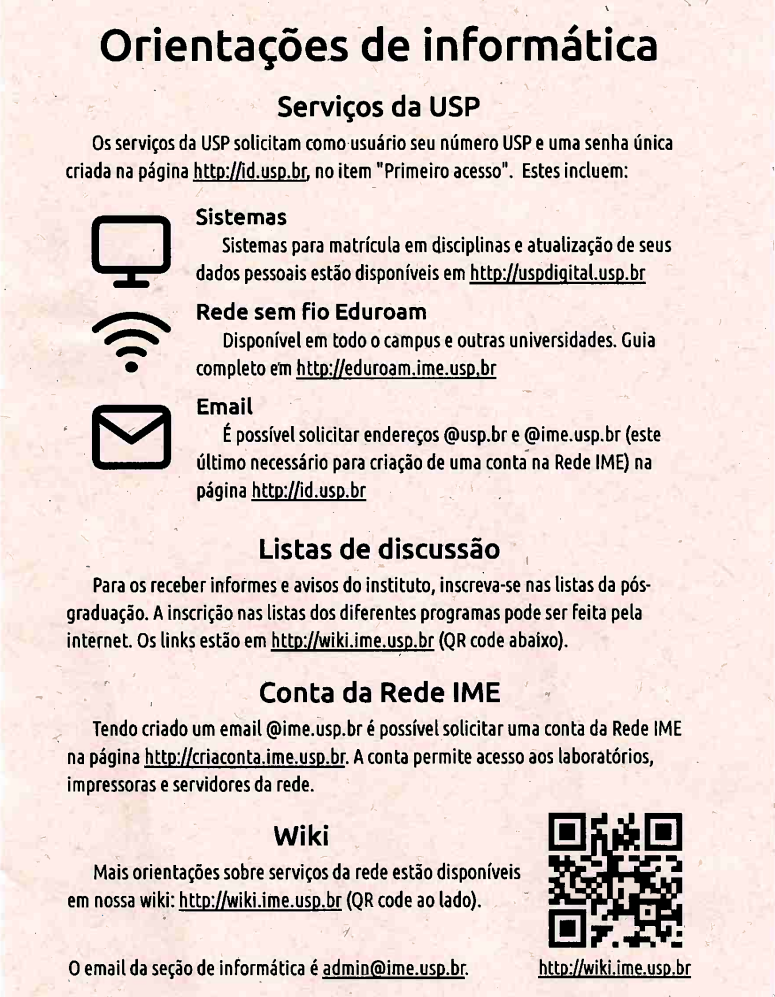
\includegraphics[width=0.5\textwidth]{imgs/email.png}
  \end{figure}

  O email institucional (tanto o \texttt{@usp.br} quanto o \texttt{@ime.usp.br}) são os meios
  oficiais de comunicação.
\end{frame}

\begin{frame}
  \textbf{Emails:}
  \begin{itemize}
    \item Email USP (\texttt{@usp.br})
    \item Email institucional (IME) (\texttt{@ime.usp.br})
  \end{itemize}
  Prestem atenção no institucional!
  \vskip 0.5cm

  \textbf{Listas de email} (em ordem decrescente de importância):
  \begin{enumerate}
    \item Lista da posmac - \texttt{g-posmac@ime.usp.br}
    \item Lista da pós-graduação - \texttt{posgraduandos@ime.usp.br}
    \item Lista do IME - \texttt{todoime@ime.usp.br}
  \end{enumerate}
  \vskip 0.5cm

  Ler email é fundamental pro programa. Não ignorem emails.
  \vskip 0.5cm

  \textbf{Redirecionem seus $n$ emails para um só!}
\end{frame}

\begin{frame}
  \frametitle{Meios de comunicação}

  \textbf{Fiquem de olho nos seguintes meios:}
  \begin{itemize}
    \item Email institucional (\texttt{@ime.usp.br}) e USP (\texttt{@usp.br})
    \item Canal de avisos
      \begin{itemize}
        \item \url{https://t.me/posmac}
      \end{itemize}
    \item Grupo de discussão
      \begin{itemize}
        \item \url{https://t.me/joinchat/Bn334VALiHokZu8eaDKjPQ}
      \end{itemize}
  \end{itemize}~\\\pause

  \textbf{Pontos importantíssimos:}
  \begin{itemize}
    \item Participem das discussões! Convívio com colegas é importante!
    \item Não tenham medo de perguntar no grupo de discussões
    \item Não tenham medo de perguntar/conversar com RDs\footnote{Afinal, eu me voluntariei pra
      isso. Se não quisesse eu não teria me candidatado. $\ddot\smile$}
    \item Participem dos grupos de extensão!
  \end{itemize}
\end{frame}

\end{document}

